\documentclass{article}
\usepackage[round]{natbib}

\usepackage{fullpage}
\usepackage{listings}
\usepackage{url}

\usepackage{graphicx}
\usepackage{color}

\lstset{language=Python}

% local definitions
\newcommand{\msprime}[0]{\texttt{msprime}}
\newcommand{\ms}[0]{\texttt{ms}}
\newcommand{\stdpopsim}[0]{\texttt{stdpopsim}}

\newcommand{\aprcomment}[1]{{\textcolor{blue}{APR: #1}}}
\newcommand{\dncomment}[1]{{\textcolor{red}{Dom: #1}}}

\begin{document}

\title{Describing demographic models is hard}
\author{A permutation of (AR, DN, JK, SG)}
\maketitle

\abstract{
Simulation plays a central role in population genomics studies. Recent years
have seen rapid improvements in software efficiency that make it possible to simulate
large genomic regions for many individuals sampled from large numbers of populations.
The increase in complexity of possible demographic models also provides additional ways
that we can get their implementation wrong. Here we describe two errors made in
defining population genetic models using the \msprime\ coalescent simulator that have
found their way into downstream analyses.
We highlight a few ways that these errors have affected analyses based on these simulations
and suggest measures that should be taken when simulating complicated demography.
}

\section{Introduction}

The \msprime\ coalescent simulator~\citep{kelleher2016efficient,kelleher2020coalescent}
is now quite widely used. The large increases in efficiency over the classical
\ms\ program~\citep{hudson2002generating} make it feasible to simulate large
samples of whole chromosomes for the first time. Another distinct advantage
of \msprime\ is the Python API that is its primary interface, greatly
increasing the flexibility and ease of use over the standard approach of
text-based command line interfaces. In particular, programs like \ms\
required users to specify cryptic command line options to describe demographic
models [JK: maybe include an example ms command line?]. Particularly for
the large models we are using today, these are not comprehensible for humans.
\dncomment{That's a pretty strong statement, might be good to give an example
or describe what it would look like (``specifying the gravel ooa model would take
10K lines of parameter specification''), or just say that its much less intuitive and
so more error prone}
The Python API for \msprime\ is a great improvement, allowing the user to
state models in a documented and reproducible manner. [JK: maybe show
the same model as described above in msprime notation?]

Implementing multi-population models of demographic history is still hard and error
prone. In this note we discuss how two poor
\dncomment{Overly harsh I think, could drop this word} design decisions
in \msprime's demography API lead
\dncomment{Also not fair I don't think. I mean Alicia's bug hints at a lack of validation that
could have happened at any stage in the pipeline, and did happen elsewhere
I believe. Could make this more positive by describing how these design choices
could be improved to reduce the chance of errors going unnoticed/eliminate
some entirely} to errors being made, which ended
up in the scientific record.
\aprcomment{You could argue it is poor API design, and I see that.. but I also
think there is something more to be said about best practices in implementing simulations,
including your own various verifications and sanity checks, and the need for robust
implementation of commonly used models (stdpopsim). I do think that in the end
the responsibility lies with the user in making sure that everything is implemented
properly.}

\section{A bad tutorial example}

To illustrate the demography API, \msprime\ included a description of a widely-used
three population Out-of-Africa model~\citep{gutenkunst2009inferring}
as part of its tutorial documentation. In this model (Fig.~\ref{fig:ooa_stats}A),
Eurasian (CEU and CHB) and African (YRI) populations split from each other in the deep past,
followed by a more recent split of European and Asian populations, with variable rates of
continuous migration between each of the populations. However, the implementation in the
\msprime\ tutorial was incorrect. Namely, at the time of the split between African and Eurasian
populations, migration between those two populations was allowed to continue for all time into the
past, resulting in population structure when there should have been just a single
randomly mating ancestral population (Fig.~\ref{fig:ooa_stats}B).

Fortunately, the effect of this error is subtle. Population sizes and structure since the time of
the split are unaffected, so that differences in expected $F_{ST}$ are negligible between
the correct and incorrect model. However, the distribution of $T_{MRCA}$ in the deep past
is distorted, and this results in an inflation of expected heterozygosity in each of the three
populations by up to $4\%$ (Fig.~\ref{fig:ooa_stats}C-G).

This model was subsequently copied
several times and used in papers [JK: do we want to estimate how
many times it was copied? A quick search on github suggests around 30
times]. \dncomment{I like this as a rough metric, like ``the number of copies
is unknown, but we found x copies on github''}

Arguably, this error occurred because of a poor
\dncomment{Again I'd go positive. If msprime is so bad, god help the rest of us.
Something like ``To model a population split in the original API, ...''?}
API design choice.
Currently, to model a population split, the user must use a MassMigration event to move
lineage from one population to another and then also remember to turn off migration
between those populations at the same time.
The release of \msprime\ 1.0 will introduce a \texttt{PopulationSplit} event, which allows
such models to be described more declaratively.
\dncomment{Strikes me as a bit programmer-centric. Maybe intuitively? Simply?}

\section{A missing parameter}

In another publication using this model~\citep{martin2017human},
a separate error was introduced: the model itself was defined as suggested
in the documentation (using somewhat more recently inferred parameters of that same
model~\citep{gravel2011demographic}) and inspected using the \msprime\
debugging tools. After these initial checks were made, however, the simulation
was performed without passing the parameter of demographic events,
so that the three populations remain separated with low levels of migration and
never merge as expected (Fig~\ref{fig:prs}A),
leading to a vast overestimate of the divergence across human populations.

In this case the error had a large effect on the simulation output and
the conclusions of the analysis. This simulation was performed to assess the
transferability of polygenic risk scores across human populations, in particular to
explore how human demographic history and population structure affects our ability
to predict genetic risk in populations of different ancestry than the originally studied
population. The resulting publication has been influential in the discussion of
health inequalities and genomics, with over 350 citations since 2017.

Unfortunately, whereas the correct model predicts a mean $F_{ST}$ of
$0.05 - 0.10$ across the three population, the simulated model generated $F_{ST}$
ranging between $0.3 - 0.6$, depending on the populations considered.
This exaggerates the role that demography plays in limiting the transferability
of genetic risk scores across populations. While this difficulty still exists
(Fig.~\ref{fig:prs}), risk prediction in each population is significantly improved
when using the correct demographic model (compare to Fig.~5 in~\citet{martin2017human}.

These errors suggests three lessons.
First, the msprime API design was poorly designed,
\dncomment{Still don't like this word. Again if msprime is poor then most bioinformatics
software is a dumpster fire. What about ``...msprime API can be adapted to
simplify common use-cases''? A bit clunky but maybe along those lines
}
requiring the user to pass
three separate parameters to specify a demographic model.
In \msprime\ 1.0 we introduce
a Demography class, which wraps these three parameters.
Thus, instead of writing
\begin{lstlisting}[frame=single]
dbg = msprime.DemographyDebugger(
  population_configurations=population_configurations,
  migration_matrix=migration_matrix,
  demographic_events=demographic_events)
dbg.print_history()
ts = msprime.simulate(
  population_configurations=population_configurations,
  migration_matrix=migration_matrix,
  demographic_events=demographic_events)
\end{lstlisting}
we would now write
\begin{lstlisting}[frame=single]
demography = msprime.Demography(
  population_configurations=population_configurations,
  migration_matrix=migration_matrix,
  demographic_events=demographic_events)
dbg = demography.debug()
dbg.print_history()
ts = msprime.simulate(demography=demography)
\end{lstlisting}

Second, testing of the final simulated data is important. This can be challenging,
because the amount of simulated data can be large. However, recent progress in
computing summary statistics from tree sequence data can make this
easier~\citep{ralph2020efficiently}.
Even if the entire simulation data cannot be easily evaluated, subsets of the data
can be examined to identify large error.

Third, open data analysis pipelines are necessary for the self-correcting nature of science.
This subtle error of large effect was only discovered through our own re-use of
the simulation pipeline developed in~\citep{martin2017human} to pursue
additional analyses on a similar topic. We identified the bug by tracing down an unexpected
result in our analysis. This error could not have been found and corrected without the open
publication of the entire analysis pipeline from the original study.

\section{Conclusions}

Defining demographic models is error prone \dncomment{Just a thought, but alternatively could say
``Demographic models are complex''}, and incorrect implementation can
impact downstream analysis and interpretation. The errors that we highlighted here have
exposed some weaknesses of the current \msprime\ API, which will be fixed in an
upcoming release. Recognition of these difficulties is also a
primary motivating factor in efforts to standardize and vet demographic model
implementation in \stdpopsim~\citep{adrion2019community}, with quality-controlled
models and simulation resources for a growing number of commonly studied species.

If you do need to implement your own demographic model, we recommend that steps are taken to
verify its correctness. A second pair of eyes (code review) or independent implementation
can go a long way in catching subtle bugs (this is the approach taken by \stdpopsim). It is also
very important to perform some basic statistical verification of the simulation, such as checking
output heterozygosity and $F_{ST}$ against expectations. If simulations are large so that
statistical validation is burdensome, you can instead simulate over a smaller genome length
and with fewer individuals to make sure basic properties hold. For example, a routine statistical
checks of $F_{ST}$ would surely
\dncomment{I'd go with either this or 'routine' but maybe not both
}
have caught the error in~\citet{martin2017human}.
\aprcomment{too snarky...? but I think it's an important point}

Finally, openness is essential. We only know about these errors because of open code and
open source development processes. \aprcomment{if we criticize the Martin paper for not
checking basic statistics, we can at least give a kudos for putting the pipeline entirely on
github here}. There must be many, many more mistakes out there, and an extra bit of care
is warranted to catch and correct such errors.

\section{Methods}

\begin{itemize}
\item Figure 1: plotted using \texttt{demography} package (\url{https://github.com/apragsdale/demography}),
allele frequency spectrum computed using \texttt{moments}~\citep{jouganous2017inferring}, and LD curves
computed using \texttt{moments.LD}~\citep{ragsdale2019models}. $F_{ST}$ and other statistics computed
from the expected AFS.
\item Figure 2: original pipeline from \url{https://github.com/armartin/ancestry_pipeline/blob/master/simulate_prs.py},
reran the experiment, with code available at \url{https://github.com/apragsdale/PRS}
\end{itemize}

\bibliographystyle{plainnat}
\bibliography{paper}

\pagebreak

\begin{figure}[ht]
\begin{center}
\makebox[\textwidth][c]{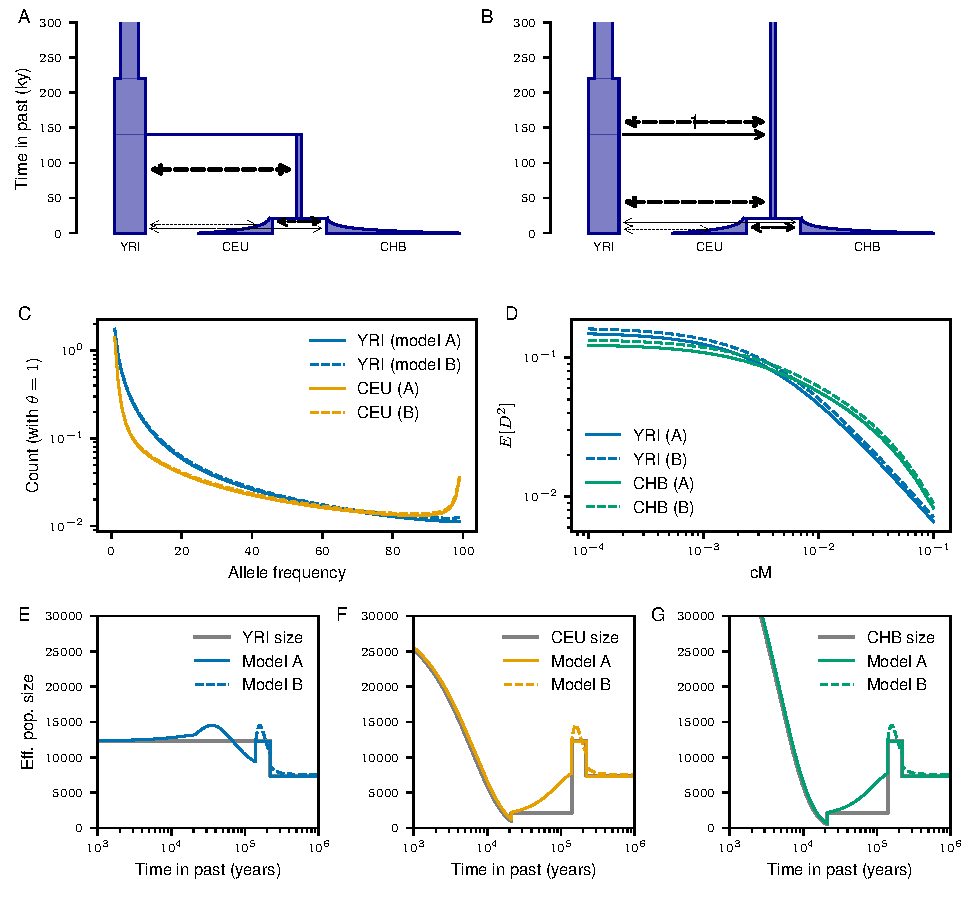
\includegraphics{figures/ooa_expected_stats.pdf}}
\caption{\textbf{Expected diversity statistics under the \citet{gutenkunst2009inferring} model}.
    \textbf{(A)} The correctly implemented model.
    \textbf{(B)} The incorrectly implemented model from the \msprime\ tutorial, with migration continuing
    into the past.
    \textbf{(C)} Marginal allele frequency spectra under the two models. Heterozygosity in the incorrect model
    is inflated by $~3.5\%$, though the general shape of the distributions are qualitatively similar.
    \textbf{(D)} Similarly, the increased heterozygosity leads to excess $D^2$, though the LD-decay is
    qualitatively similar between models.
    \textbf{(E-G)} True size history for each population plotted against the expected size history from
    the expected inverse coalescence rates.
}
\label{fig:ooa_stats}
\end{center}
\end{figure}

\begin{figure}[ht]
\begin{center}
\makebox[\textwidth][c]{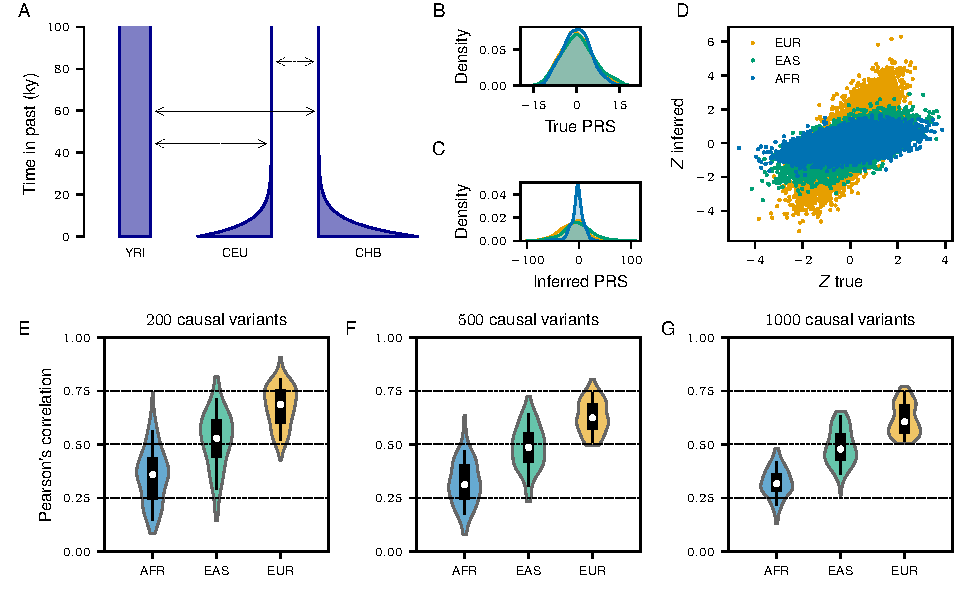
\includegraphics{figures/prs_fig.pdf}}
\caption{\textbf{The transferability of PRS under neutrality}.
    \textbf{(A)} In~\citet{martin2017human}, the simulated demographic model did not apply demographic
    events in the past, so continental populations were simulated as isolated with low levels of migration
    for all time.
    \dncomment{Might have been on your todos below but would help I think to have the correct model
    drawn out too (see now that you did in fig 1. I'd at least point to that to highlight the difference)}
    \textbf{(B-G)} We repeated the simulation experiment in~\cite{martin2017human} using the correct
    demographic model and found that risk prediction was greatly improved over what was originally
    reported in all three populations.
    \aprcomment{directly compare to figure 5 in the original paper}
    \aprcomment{to do: fill in caption}
}
\label{fig:prs}
\end{center}
\end{figure}


\end{document}
